% !TeX spellcheck = en_GB
\documentclass[journal,10pt]{IEEEtran}

% *** CITATION PACKAGES ***
%
\ifCLASSOPTIONcompsoc
  \usepackage[nocompress]{cite}
\else
  % normal IEEE
  \usepackage{cite}
\fi
% *** GRAPHICS RELATED PACKAGES ***
\ifCLASSINFOpdf
	\usepackage[pdftex]{graphicx}
\else
	\usepackage[dvips]{graphicx}
\fi
\usepackage{amsmath}
\usepackage{amssymb}
\usepackage{bm}
\usepackage{textcomp}
%
%\usepackage{algorithmic}
%\usepackage{algorithm}

%\usepackage{algorithmicx}

\usepackage[linesnumbered,ruled,vlined]{algorithm2e}

%\usepackage[noend]{algpseudocode}
\usepackage{array}
\ifCLASSOPTIONcompsoc
  \usepackage[caption=false,font=footnotesize,labelfont=sf,textfont=sf]{subfig}
\else
  \usepackage[caption=false,font=footnotesize]{subfig}
\fi
%\usepackage{fixltx2e}
% \usepackage{stfloats}
\usepackage{tikz}
\usepackage{cite}
%\usepackage{dblfloatfix}
\usepackage{url}
\usepackage{comment}
\usepackage{color}
\usepackage{subfloat}
%\usepackage[automake, acronym]{glossaries}
\usepackage{multirow}
\usepackage[colorinlistoftodos,prependcaption,textsize=tiny]{todonotes}
%\usepackage{widetext}
%\usepackage{subcaption}
%\usepackage{subfigure}
\usepackage[keeplastbox]{flushend}
\newtheorem{theorem}{Theorem}

%configure hyphenation
\lefthyphenmin8
\righthyphenmin8
\hyphenation{op-tical net-works semi-conduc-tor}

\newcommand{\newnote}[2]{\todo[linecolor=#1,backgroundcolor=#1!25,bordercolor=#1]{#2}}
\newcommand{\snotesc}[1]{\newnote{red}{SC: #1}}
\newcommand{\snoteam}[1]{\newnote{blue}{AM: #1}}

\newcommand{\notesc}[1]{\snotesc{}\textcolor{red}{SC: #1}}
\newcommand{\noteam}[1]{\snoteam{}\textcolor{blue}{AM: #1}}

\newcommand{\blue}[1]{\textcolor{blue}{#1}}
\newcommand{\red}[1]{\textcolor{red}{#1}}

\newcommand{\lastaccessedtoday}{Last accessed: \today}
\newcommand{\etal}{{\it et. al.} }

\let\oldnl\nl% Store \nl in \oldnl
\newcommand\nonl{%
	\renewcommand{\nl}{\let\nl\oldnl}}

\setcounter{figure}{1} 
\begin{document}
\begin{figure}
	\captionsetup[subfigure]{}
	\begin{center}
		\subfloat[\label{fig:averageQuality}]{
			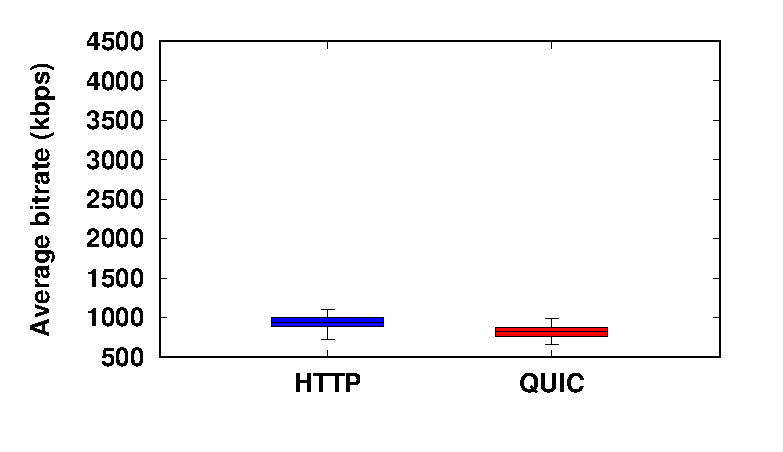
\includegraphics[width=.49\linewidth]{rimg/AQ_box}
		}
		\subfloat[\label{fig:averageQuality_n}]{
			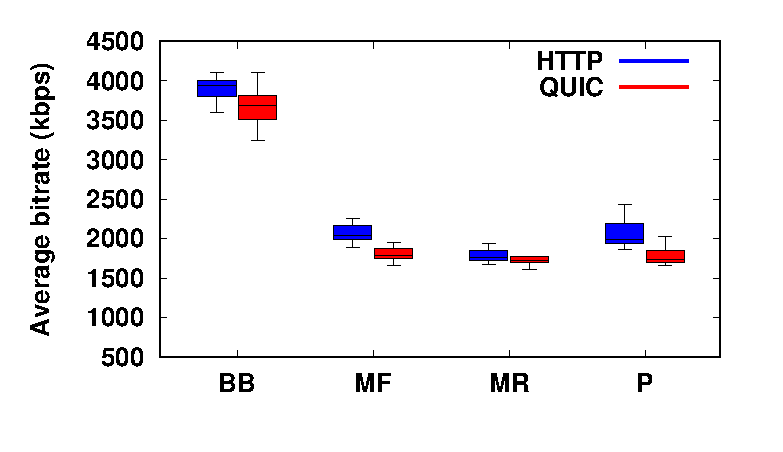
\includegraphics[width=.49\linewidth]{rimg/bitrate_box}
		}
	\end{center}
	\caption{(a) Average Playback Video Quality, (b) Average Playback Video Quality for Different ABR Techniques}
\end{figure}

\begin{figure}
	\captionsetup[subfigure]{}
	\begin{center}
		\subfloat[\label{fig:averageQualityVariation}]{
			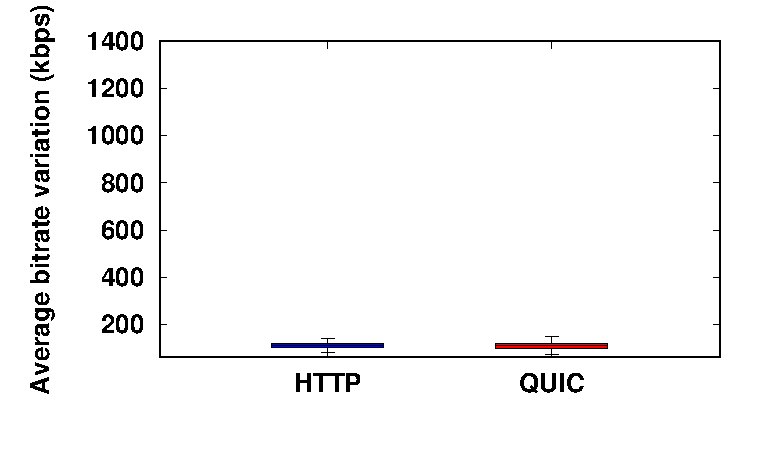
\includegraphics[width=.49\linewidth]{rimg/AQV_box}
		}
		\subfloat[\label{fig:averageQualityVariation_n}]{
			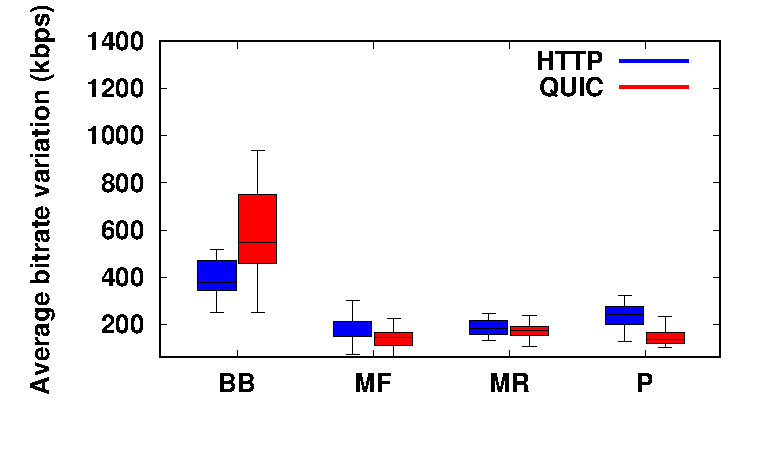
\includegraphics[width=.49\linewidth]{rimg/smooth_box}
		}
	\end{center}
	\caption{(a) Average Playback Quality Variation, (b) Average Playback Quality Variation for Different ABR Techniques}
\end{figure}

\begin{figure}
	\captionsetup[subfigure]{}
	\begin{center}
		\subfloat[\label{fig:RebufferTime}]{
			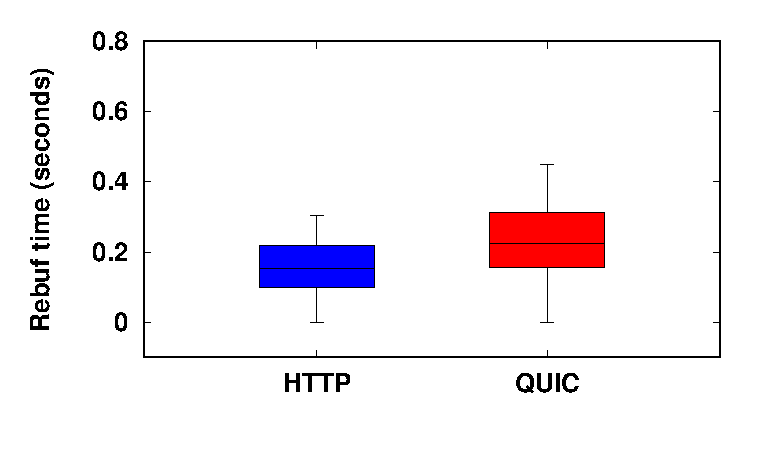
\includegraphics[width=.49\linewidth]{rimg/RT_box}
		}
		\subfloat[\label{fig:RebufferTime_n}]{
			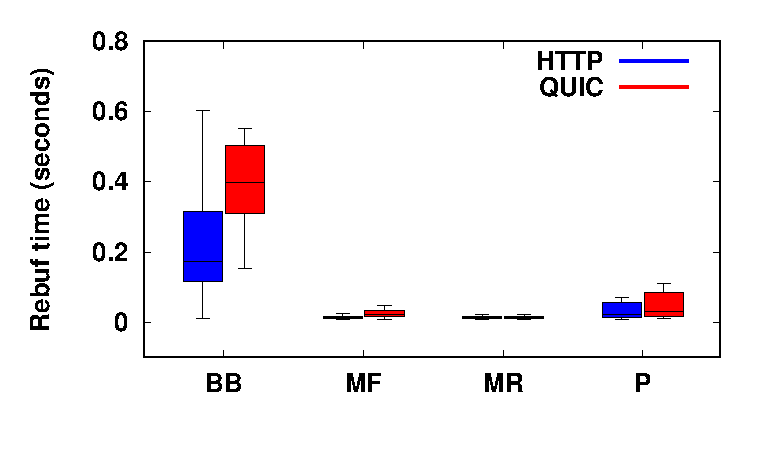
\includegraphics[width=.49\linewidth]{rimg/rebuf_box}
		}
	\end{center}
	\caption{ (a) Rebuffering Time, (b) Rebuffering Time for Different ABR Techniques}
\end{figure}

\begin{figure}
	\captionsetup[subfigure]{}
	\begin{center}
		\subfloat[\label{fig:QOE}]{
			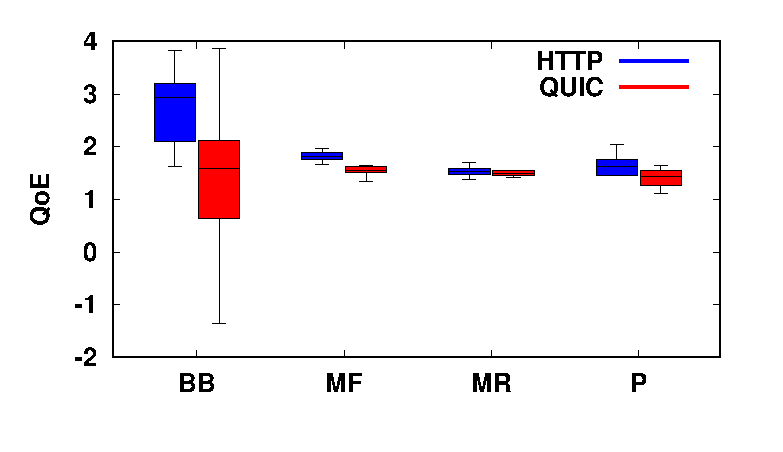
\includegraphics[width=.49\linewidth]{rimg/QOE_box}
		}
		\subfloat[\label{fig:QOE_n}]{
			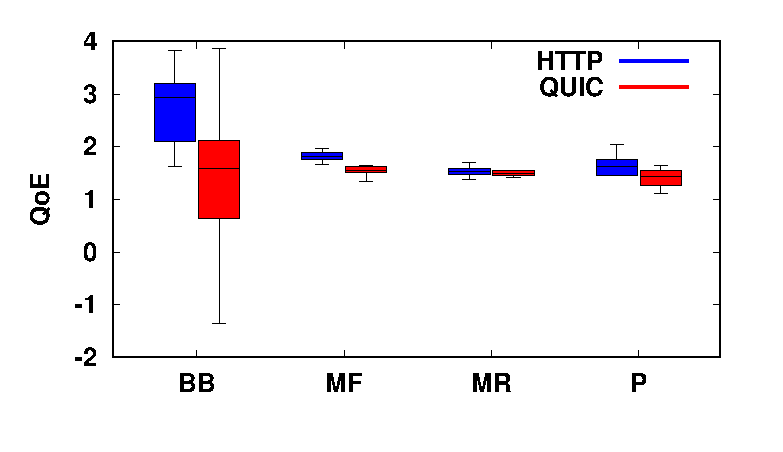
\includegraphics[width=.49\linewidth]{rimg/qoe_box}
		}
	\end{center}
	\caption{(a) Overall QoE, (b) Overall QoE for Different ABR Techniques}
\end{figure}



\end{document}


